% Ubah judul dan label berikut sesuai dengan yang diinginkan.
\section{Experiment Setup}
\label{sec:experiment-setup}

% Ubah paragraf-paragraf pada bagian ini sesuai dengan yang diinginkan.

\subsection{Model Development Phase}
\label{subsec:model-development-phase}
\par We use a public dataset available on Kaggle, comprising 30,905 raw queries of SQLi attacks and benign traffic from different websites \cite{SQLiDataset}. With a 63:37 ratio of safe to malicious query, we consider this case as an imbalanced dataset. In reality, a malicious query occurs less than a safe query. Thus, using the F1 score to evaluate the model is more suitable for this case. A stratified train-test split with a ratio of 80:20 is performed on the data.
\par A fixed-length sequential data is required to train the LSTM. Based on Figure \ref{fig:eda_violinplot_n_token_query}, we set the maximum length of a query to be 30 tokens, which satisfies more than 90\% of the training data. If a query is more than 30 tokens, the query will be pre-truncated, and if less than 30 tokens, the query will be pre-padded with zero vectors. Also, several tokens only occur once in the dataset, which can be assumed as noise tokens. Hence, based on Figure \ref{fig:eda_lineplot_token_cutoff_freq.png}, we set the cut-off frequency to two. In other words, all tokens that only occur once will be treated as an out-of-vocabulary token.

\begin{figure} [ht]
  \centering
  % Ubah sesuai dengan nama file gambar dan ukuran yang akan digunakan.
  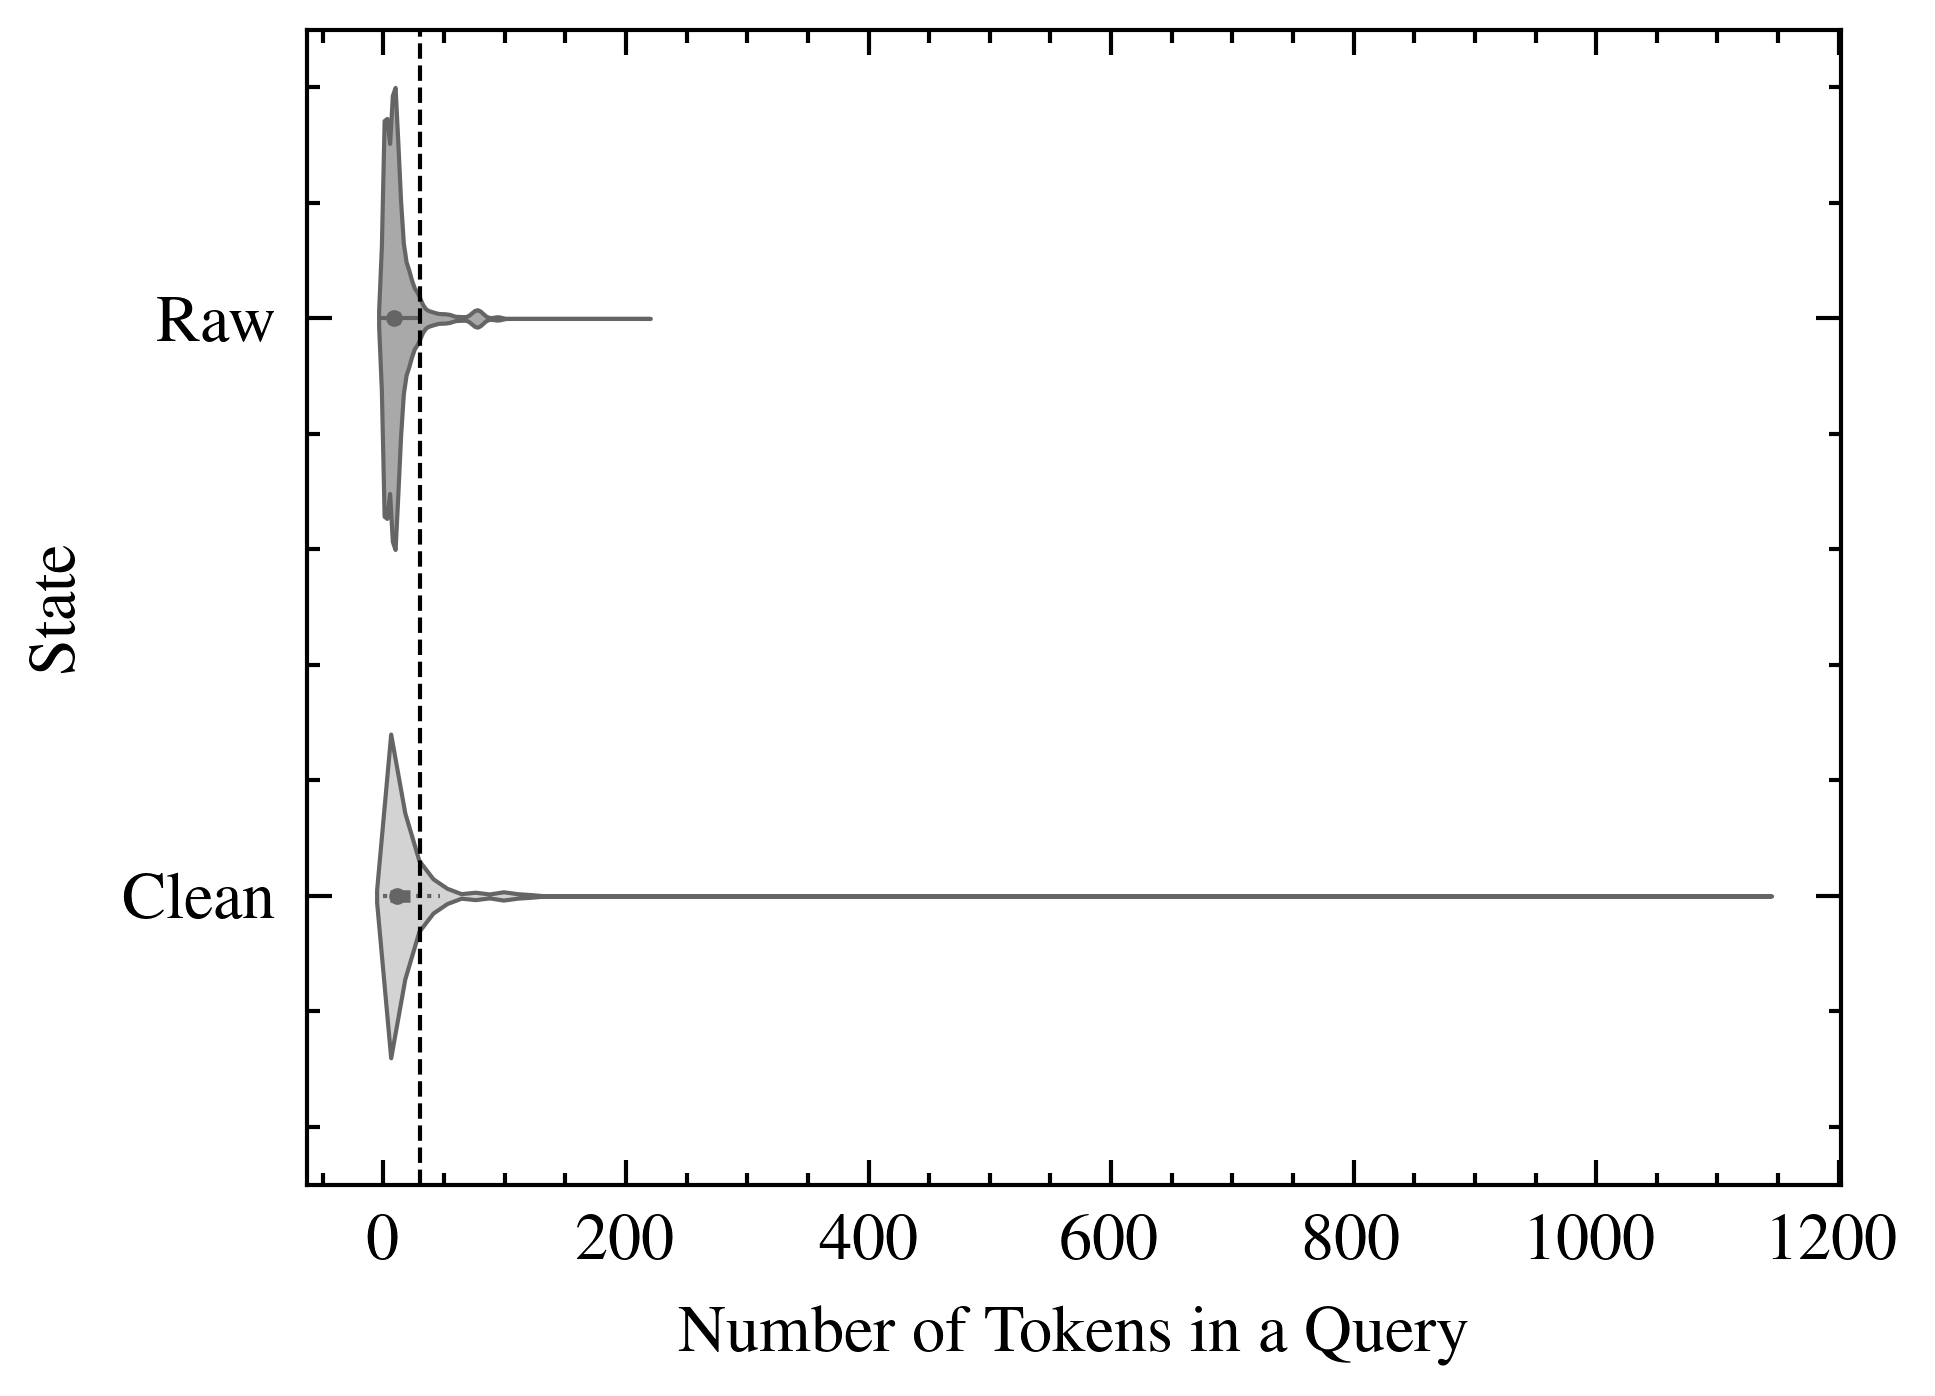
\includegraphics[width=0.4\textwidth]{image/eda_violinplot_n_token_query.png}

  % Ubah sesuai dengan keterangan gambar yang diinginkan.
  \caption{The distribution of the number of tokens in a query}
  \label{fig:eda_violinplot_n_token_query}
\end{figure}

\begin{figure} [ht]
  \centering
  % Ubah sesuai dengan nama file gambar dan ukuran yang akan digunakan.
  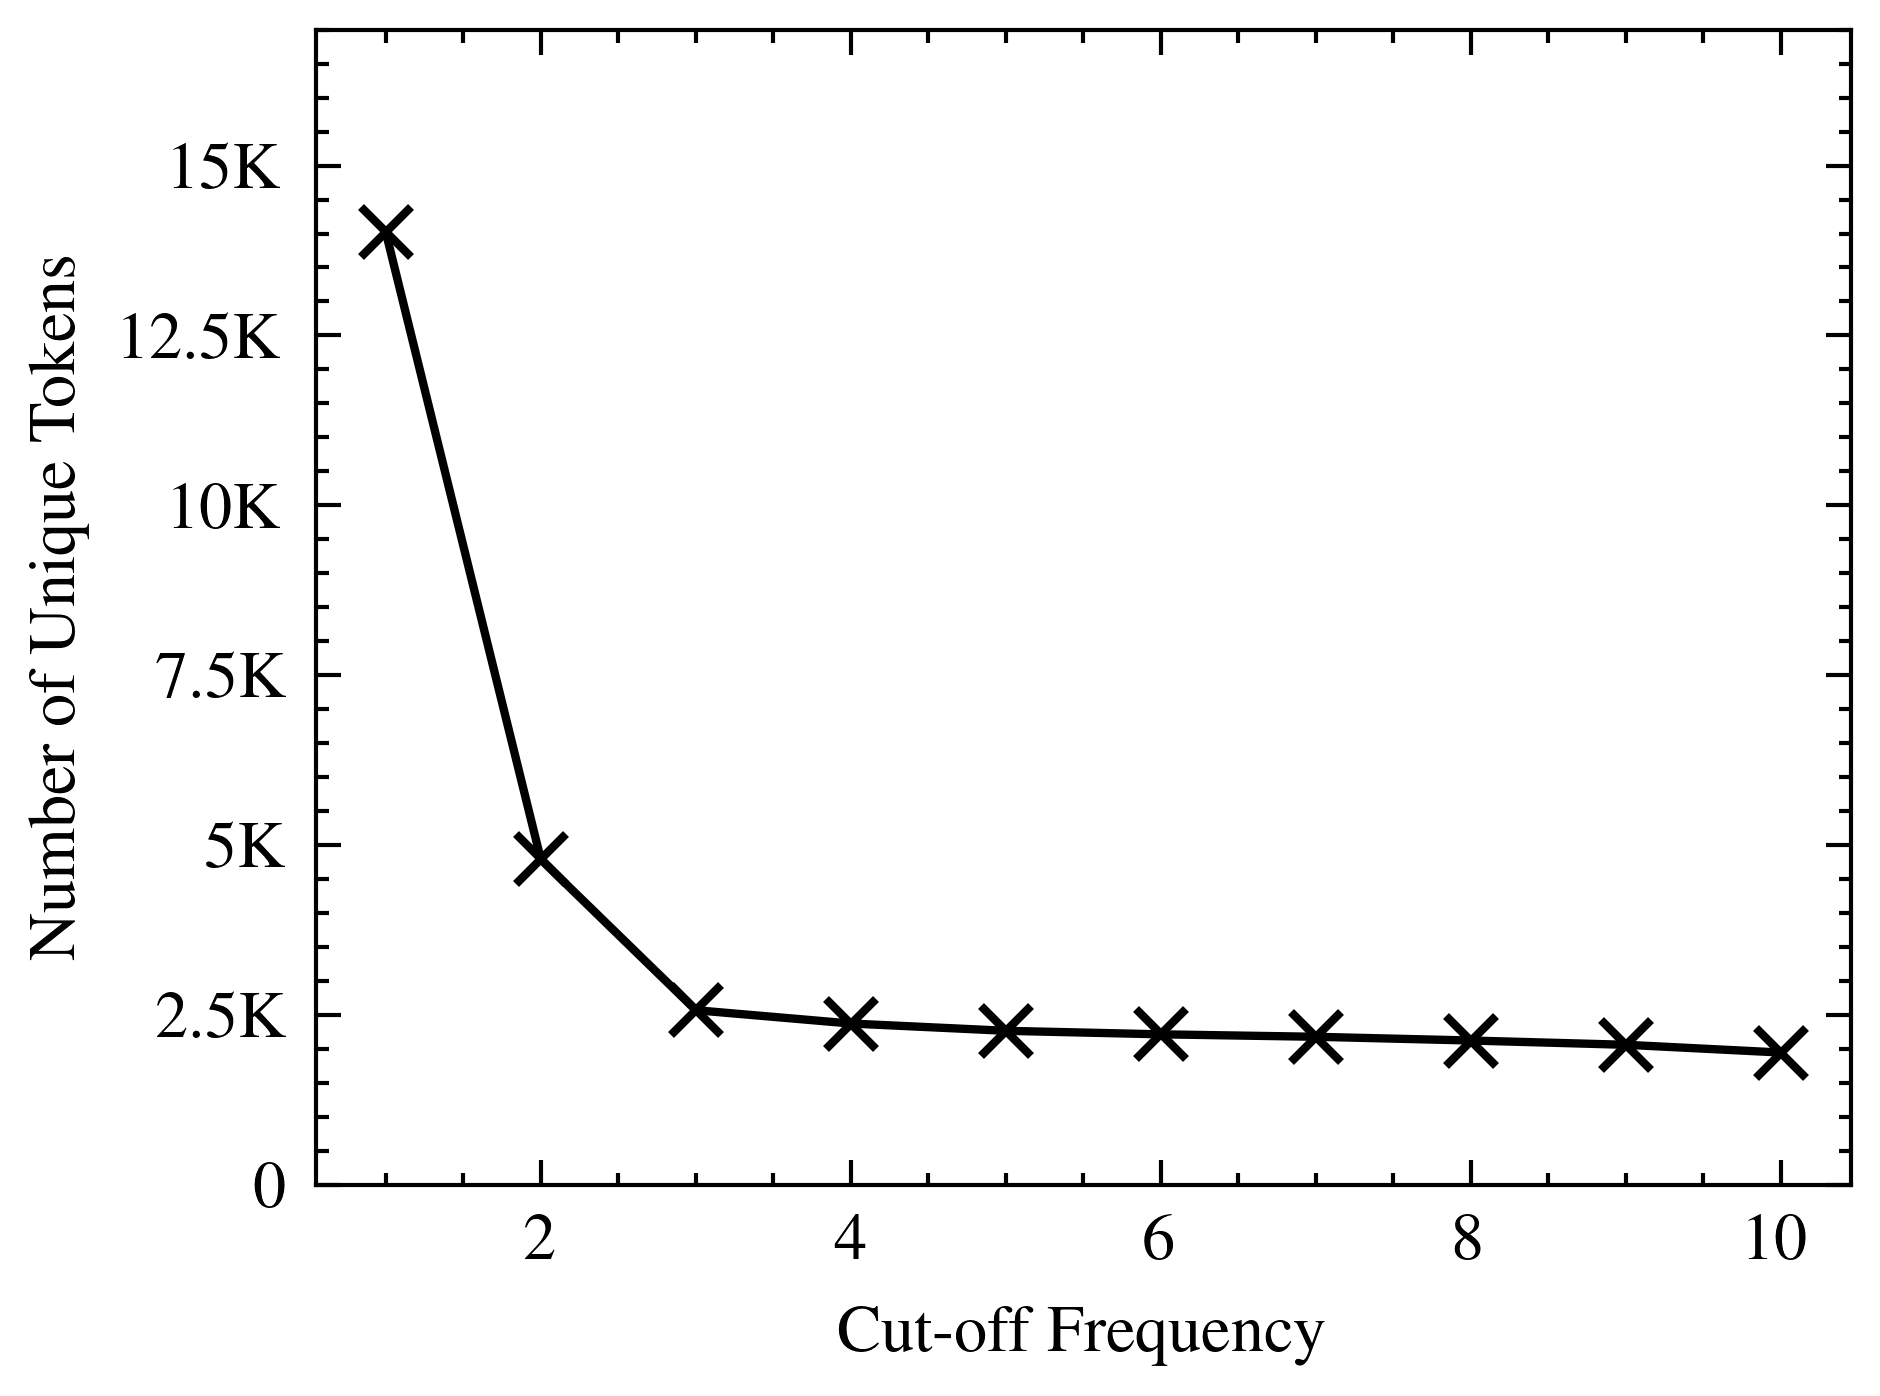
\includegraphics[width=0.35\textwidth]{image/eda_lineplot_token_cutoff_freq.png}

  % Ubah sesuai dengan keterangan gambar yang diinginkan.
  \caption{Token cut-off frequency}
  \label{fig:eda_lineplot_token_cutoff_freq.png}
\end{figure}

\par The "best" LSTM model is obtained by searching the hyperparameter out of 18 combinations (shown in Table \ref{tab: hyperparameter-lstm}) that achieve the highest mean F1 score in the validation data using 5-fold cross-validation. For comparison, we also trained the data using ten supervised machine-learning algorithms using default hyperparameters from scikit-learn \cite{scikit-learn}:
\begin{itemize}[
    \setlength{\IEEElabelindent}{\dimexpr-\labelwidth-\labelsep}% Wrapping of text beyond first line of \item
    \setlength{\itemindent}{\dimexpr\labelwidth+\labelsep}% identation for each new \item
    \setlength{\listparindent}{\parindent}% Restore regular paragraph indentation
  ]
  \item Linear classifier: Logistic regression, Linear discriminant analysis, SVM linear
  \item Non-linear classifier: KNN, Naive Bayes, SVM using RBF kernel
  \item Tree-based model: Decision tree (depth = 50), Random forest (depth = 50), Ada boost, Gradient boost
\end{itemize}

\par Each model's prediction time is also considered because, in a real-world application, the model has to be as fast as possible to predict the user query. Ideally, we want a predictive model with a maximum F1 score and minimum prediction time. We measured the prediction time in milliseconds per query by predicting the validation data during 5-fold cross-validation. Table \ref{tab: specifications} shows the hardware and software specifications used for our experiments.

\begin{table}[!htp]\centering
\caption{Hyperparameter combinations for LSTM training}\label{tab: hyperparameter-lstm}
\scriptsize
\begin{tabular}{lrrr}\toprule
\textbf{Component} & \textbf{Hyperparameter} & \textbf{Combinations} \\\midrule
\row{Input layer} & Input length &[30] \\
&Embedding dimension &[32, 64, 128] \\
\row{Hidden layer} & Num of layers and nodes per layer &[[32], [32, 32], [32, 32, 32]] \\
&Layer type (direction) & [Uni-LSTM, Bi-LSTM] \\
\row{Learning} & Optimizer & [adam] \\
&Learning rate &[0.001] \\
&Epoch &[10] \\
&Validation &[0.2] \\
\bottomrule
\end{tabular}
\end{table}

\begin{table}[!htp] \centering
\caption{Hardware and software specifications}\label{tab: specifications}
\resizebox{.5 \textwidth}{!}{%
\begin{tabular}{lll}
\midrule
\textbf{Component} &\textbf{Sub-component} &\textbf{Specification} \\\midrule
\multirow{}{}{Hardware} 
&Memory &16,184 MB RAM \\
&Processor &Intel(R) Core(TM) i7-10510U\\
& &CPU @ 1.80GHz (8 CPUs), ~2.3GHz \\
\multirow{}{}{Software} 
&Python &3.10.6 \\
&tensorflow \cite{tensorflow2015-whitepaper} &2.10.0 \\
&scikit-learn \cite{scikit-learn} &1.1.2 \\
&scikeras  \cite{scikeras} &0.9\\
& Operating System & Windows 11 Home Single \\
& & Language 64-bit (10.0, Build 22621)\\\midrule
\end{tabular}%
}
\end{table}

\subsection{Prediction Phase}
\label{subsec:prediction-phase}
\par We implemented the SQLi detection on the user login scenario. The prototype application is built using Flask, a Python-based web framework. However, Flask does not have a database storage system, so we implemented it using SQLite. Both Flask and SQLite are available in Python, making it easier to integrate them with the model we have built. For the SQLite database, we set it up as a no-SQL database, as it is only a prototype and there is no need for a relational database.

\par We used a list of 386 lines of SQLi attacks created by Daniel Miessler \cite{seclist} for the keyword filtering. There are three categories of blacklist according to his project:
\begin{itemize}[
    \setlength{\IEEElabelindent}{\dimexpr-\labelwidth-\labelsep}% Wrapping of text beyond first line of \item
    \setlength{\itemindent}{\dimexpr\labelwidth+\labelsep}% identation for each new \item
    \setlength{\listparindent}{\parindent}% Restore regular paragraph indentation
  ]
  \item General blind SQLi, when the attacker queries yes and no questions and tries to gain information using those queries,
  \item General SQLi, when the attacker attempts to gain admin access, and
  \item Quick SQLi, when the attacker attempts to make the username and password input query equal to TRUE.
\end{itemize}
\par We combined all three blacklists into a Blacklist table stored in SQLite. Furthermore, the trained model is saved as a joblib pipeline, with no mandatory dependency on the libraries used to create the model itself besides Python. We combined keyword filtering and model pipeline to prevent SQLi attacks using the two-step prevention described in Table \ref{tab:decisionmaking}.

\par Table \ref{tab: sample-input} illustrates how our prototype application responds in different scenarios. The only case where the user would gain access to their account is when they input a non-malicious query in both the username and password fields and matched with the User table. Note that in a real-world implementation, we would output the same message for cases 1 and 2.
\begin{table*}[!htp]\centering
\caption{Sample Input Cases}\label{tab: sample-input}
\scriptsize
\begin{tabular}{lrrrr}\toprule
\textbf{Case} &\textbf{User Input Scenario} &\textbf{Sample Input} &\textbf{Message} \\\midrule
\multirow{}{}{1} &\multirow{}{}{Malicious query} &username: admin' or 1=1 &\multirow{}{}{“Your request is rejected"} \\
& &password: 12345678 & \\
\multirow{}{}{2} &\multirow{}{}{Non-malicious query but not exists in the User table} &username: a &\multirow{}{}{"Username or Password is incorrect"} \\
& &password: 12345678 & \\
\multirow{}{}{3} &\multirow{}{}{Non-malicious query and exists in the User table} &username: FNietzsche &\multirow{}{}{"Logged In"} \\
& &password: 12345678 & \\
\bottomrule
\end{tabular}
\end{table*}

